% LCFM @ NeurIPS 2026 camera-ready. Long paper: main text <= 8 pages.
%
% Build: cd manuscript/lcfm && tectonic main.tex
%
% TEMPLATE. The official NeurIPS 2026 package (neurips_2026.sty), copied from the reviewed
% submission's own directory, with the same option set it used plus [final]: the [final]
% option is what makes this a camera-ready copy, and the style then prints the author block
% and drops the anonymization. No proxy: the style file is the submission's own.
%
% Author block: restored from the reviewed submission's own camera-ready block
% (commit 44038b2). See results/lcfm/FINAL_REPORT.txt for the one discrepancy with the
% arXiv long version's affiliation line.
%
% EM DASHES. House style: none. Every em dash was removed from this file, whether written
% as a run of three hyphens or as the Unicode character, and the same was done to the figure
% script and to the tables this paper includes. En dashes are kept where they belong, in
% numeric ranges.
%
% NUMBERS. Every number in the main text carries a % SRC: comment naming the artifact it
% comes from, and all of them are generated from the CSVs by scripts/lcfm_figures.py.

\documentclass{article}

\usepackage[dblblindworkshop, final]{neurips_2026}
\workshoptitle{Workshop on Long Context Foundation Models (LCFM) @ NeurIPS 2026}

\usepackage[utf8]{inputenc}
\usepackage[T1]{fontenc}
\usepackage[hidelinks]{hyperref}
\usepackage{url}
\usepackage{booktabs}
\usepackage{amsfonts}
\usepackage{amsmath}
\usepackage{amssymb}
\usepackage{textcomp}
\usepackage{microtype}
\usepackage{xcolor}
\usepackage{graphicx}
\usepackage{enumitem}

\graphicspath{{../../results/lcfm/figs/}{../../figures/}{./}}
\urlstyle{tt}
\Urlmuskip=0mu plus 1mu
\emergencystretch=3em

\newcommand{\src}[1]{\texttt{#1}}

\author{%
  Aman Kesarwani \\
  Independent Researcher \\
  \texttt{amankesarwani@berkeley.edu} \\
}

\title{What Limits Speculative Decoding at a Million Tokens?\\
       Greedy Loops, Rotary Stretching, and the Ring's Decode Step}

\begin{document}
\maketitle

\begin{abstract}
Speculative decoding's short-context speedups do not survive million-token inference, and the
reason is not the mechanism the technique's own literature would predict. We report three
scientific findings and two systems measurements on 8$\times$A100 80\,GB SXM4 with FP4 weights
and an NF4 KV cache. \emph{First}, the acceptance such campaigns report is measured on
degenerate text: under greedy decoding 9 of 10 rows in the released long-context first-window
audit loop and 1 of 10 temperature-arm rows does, against 1 of 83 sampled rows at $T{=}0.7$. A
greedy draft accepts a loop trivially, so a greedy acceptance number measures the text.
\emph{Second}, stretching the rotary basis of a model that ships the scaling dictionary costs a
quarter of speculative acceptance for almost no perplexity: at 128\,k, acceptance falls from
$0.7272$ to $0.5336$ and $0.5006$ while the paired perplexity ratio moves by $+0.05\%$ and
$+1.56\%$. Acceptance is not a proxy for perplexity. \emph{Third}, a natively 1M-trained target
stays coherent at 1\,M, within $9.5\%$ of its own 128\,k perplexity on the exactly aligned
book. \emph{Fourth}, our ring's decode bottleneck was the per-token key/value rotation: 256
rounds per token at a fixed ${\sim}10.3$\,ms each regardless of payload, so per-round latency
and not bandwidth. Removing it is worth $2.80$ to $4.37\times$ decode-only with speculation and
$3.30$ to $5.32\times$ without. \emph{Fifth}, speculation still pays $2.01$ to $2.29\times$ on
top, and the matched 1\,M acceptance is unchanged ($-0.1\%$). Against vLLM at bf16 with greedy
decoding, which is not a precision-matched comparison, our prefill beats its entire run by
$1.92$ to $2.56\times$ while its decode stays $130$ to $162\times$ faster per token than
ours.
\end{abstract}

\section{Introduction}
\label{sec:intro}

Serving a million-token context on eight commodity GPUs forces two problems at once. The KV
cache does not fit, which ring attention \citep{liu2023ringattention} solves by sharding the
sequence dimension and rotating key/value blocks around the ranks. And every generated token
still costs a full forward pass, which speculative decoding
\citep{leviathan2023fast,chen2023accelerating} attacks by having a small draft propose several
tokens and verifying them with one target forward. Combining the two is the obvious systems
move, and the interesting question is what happens to the second mechanism once the first is
in place.

We built \textbf{RASD}, a ring-attention engine with an NF4 KV cache, chunked updates, an
attention-sink prefix, rotary scaling where a target needs it, and speculative verification,
and asked whether speculation still pays at 1\,M. The measurements kept saying that something
else was wrong, so the findings below lead with the science and close on our own engine.

\paragraph{F1. Acceptance and perplexity dissociate under rotary stretching.}
On \texttt{meta-llama/Llama-3.1-8B}, a model that ships the \texttt{rope\_scaling} dictionary
the intervention edits, stretching the rotary basis at 128\,k moves paired perplexity by
$+0.05\%$ (factor 16) and $+1.56\%$ (factor 32) while speculative acceptance falls from
$0.7272$ to $0.5336$ and $0.5006$. The arms differ in nothing but \texttt{rope\_factor} and
the direction holds on five books of five. Position scaling is judged by perplexity; here it
is nearly free by that measure and expensive by the measure a speculative decoder cares
about.
% SRC: results/mlsys/sampling_session/session_a_ROPE_SAMP_{NATIVE,F16,F32}_SPEC.csv; session_a_rope_fix_gate.csv

\paragraph{F2. Greedy acceptance numbers at long context are measured on degenerate text.}
Under greedy decoding, 9 of 10 rows in the released long-context first-window audit degenerate
into repetition, and 1 of 10 in the later temperature arms does, against 1 of 83 sampled rows
at $T{=}0.7$; that one row is a rotary variant and \S\ref{sec:res-degeneracy} names it. A
greedy acceptance number therefore measures the degeneracy and not the agreement between draft
and target, which is why this campaign moved to sampling and why every row here carries an
explicit periodicity verdict.
% SRC: results/mlsys/natural_f1_128k_first_window.csv; seeds_ablations/repetition_SA_TEMP_{0,1_0}_128K_SPEC.csv; scripts/lcfm_figures.py Fig C census

\paragraph{F3. A natively long-context target is coherent at 1\,M.}
On the one exactly aligned book, the target's own perplexity at 1\,M is $1.805$ against
$1.649$ at 128\,k, a $+9.5\%$ move; on the two books that share 91 to 95\% of their scored
tokens it is within $1.1\%$. Long context is therefore not intrinsically hostile to
speculation, which is what made the two systems findings below worth chasing.
% SRC: results/mlsys/sampling_session/QUALITY_FIX_1M_* vs QUALITY_FIX_128K_*; alignment.csv

\paragraph{F4. Our ring's decode step was the key/value rotation.}
At 128\,k each decode token needs 8 rotations over 32 layers, so 256 rounds of a
\texttt{batch\_isend\_irecv} ring. A bare-process benchmark of that primitive, with no model
attached, shows every payload costs the same ${\sim}10.3$\,ms: 10.3124\,ms for 4\,KB against
10.3462\,ms for 266\,MB, a 66{,}000$\times$ payload range with a $0.4\%$ spread. The cost is
latency per round. Removing the rotation with decode-side context parallelism, which is prior
work \citep{yang2024contextparallelism}, is worth
\textbf{2.80$\times$ / 3.77$\times$ / 4.37$\times$} decode-only with speculation and
\textbf{3.30$\times$ / 4.26$\times$ / 5.32$\times$} without it at 128\,k / 512\,k / 1\,M on
matched (seed, book) cells, and the speedup grows with context, which is what a
context-independent per-round cost predicts.
% SRC: results/mlsys/decode_df/ring_bench/ringbench.csv; results/mlsys/RESULTS_OCT.md section 10.2b

\paragraph{F5. Speculation still pays, and the 1\,M acceptance is unchanged.}
With the rotation gone, speculation is worth $2.01\times$ / $2.29\times$ / $2.20\times$
decode-only over the same engine's target-only path at 128\,k / 512\,k / 1\,M. Acceptance at
1\,M under the fixed engine is $-0.1\%$ against the corrected old-engine baseline over 13
matched cells, and the target-only token stream from the fixed kernel is bit-identical to the
ring's for twelve tokens before diverging where the baseline's own top-2 margin is 0.0000, so
the speedups are not bought with a different model.
% SRC: results/mlsys/RESULTS_OCT.md sections 10.2, 10.3, 10.7

\paragraph{What this paper does not claim.} The rotation-free decode kernel is prior work,
cited for the technique and never claimed: Meta's context parallelism in its pass-KV and
pass-Q forms \citep{yang2024contextparallelism} and vLLM's Decode Context Parallelism
\citep{lee2026dcp}. Our contribution is the diagnosis and the measurement. The comparison
against vLLM is \textbf{not precision-matched} (\S\ref{sec:res-vllm}).

\section{Background and Related Work}
\label{sec:related}

\paragraph{Long-context attention.} Ring attention \citep{liu2023ringattention} shards the
sequence across ranks and pipelines exact attention through a ring of exchanges, so per-rank
memory is independent of sequence length, with FlashAttention-2
\citep{dao2023flashattention2} as the local kernel. Its published evaluation is a prefill
story; what a decode step costs once every layer's key/value shard must visit every rank is
what \S\ref{sec:res-decode} measures.

\paragraph{Decode-side context parallelism (prior work).} The decode-phase gap is closed in
the literature, and we cite rather than claim it. Meta's context-parallel report
\citep{yang2024contextparallelism} describes ring-context parallelism for million-token
inference in pass-KV and pass-Q forms: instead of rotating every key/value block for each new
query, a rank attends to the blocks it already holds and the partials are combined, with the
query replicated in the pass-Q form. vLLM's Decode Context Parallelism \citep{lee2026dcp} is
the production implementation, motivated by KV memory that tensor parallelism cannot shard
once the head count is small. We adopt the pass-Q form as \emph{split-KV}.

\paragraph{Speculative decoding.} \citet{leviathan2023fast} and \citet{chen2023accelerating}
established draft-and-verify: a small model proposes $\gamma$ tokens, the target verifies them
in one pass, and the longest accepted prefix is kept with a residual resample for the rejected
position. Acceptance $\alpha$ is the fraction the target accepts and the single-device speedup
is roughly $(1-\alpha^{\gamma+1})/(1-\alpha)$; \citet{cai2024medusa} removed the separate
draft model with multi-head prediction. All of it is evaluated at short context, and the
interaction with a distributed KV cache is the setting here.

\paragraph{KV compression and position scaling.} NF4 quantization
\citep{dettmers2023qlora} shrinks the cache and an attention-sink prefix
\citep{xiao2024streamingllm} stabilises it. Rotary embeddings \citep{su2024rope} are stretched
past a model's training window by YaRN \citep{peng2023yarn}, an intervention normally
validated by perplexity alone; \S\ref{sec:res-rope} shows what that misses.

\section{System and Setup}
\label{sec:setup}

\paragraph{RASD in brief.} RASD runs on one node of 8$\times$A100 80\,GB SXM4, with the target
and a 1.3B draft on every rank. The KV cache is NF4 with chunked updates and a bf16
attention-sink prefix of the first 128 tokens on rank 0; the input is sharded across ranks;
attention is ring attention with FlashAttention-2 in each local block; the weights are
\textbf{FP4}, since NF4 is the KV codec, a distinction the reviewed version blurred. At 1\,M
the system peaks at \textbf{41.2\,GiB allocated per rank} over the ranks with 69\,GiB
reserved, where the vanilla HuggingFace stack runs out of memory at 128\,k single-rank.
Rotary scaling is applied at a fixed factor 8 at 8\,k and above and not at all below that,
anchored on each context's own length because the \texttt{transformers} version in use ignores
\texttt{original\_max\_position\_embeddings}.
% SRC: results/mlsys/RESULTS_OCT.md section 1; results/mlsys/LCFM_RECONCILE.md (AUDIT E7/E8/E18/E19)

\paragraph{Targets.} Two appear. The long-context campaign runs
\texttt{gradientai/Llama-3-8B-Instruct-Gradient-1048k}, trained to a 1\,M window, so nothing is
stretched; the rotary intervention of \S\ref{sec:res-rope} runs
\texttt{meta-llama/Llama-3.1-8B}, which ships the scaling dictionary under test, with a
tokenizer-sharing draft. A ceiling test on \texttt{meta-llama/Llama-2-7b-hf}, the 4\,k-window
model the engine was first built on, is a capability reference only and no ratio here uses it;
it is detailed in Appendix~\ref{app:evidence}.
% SRC: results/lcfm/CAMERA_READY_KIT.md section 3e (limitation 4)

\paragraph{Protocol of every reported result.} Prompts are PG-19 narrative
\citep{rae2019pg19}, five books, windowed so each rung's scored continuation ends at the same
document position as the 1\,M rung, with the alignment verified from
\texttt{continuation\_sha256} and the recorded offsets rather than from a pool name. Decoding
is $T{=}0.7$ sampling, 128 new tokens, $\gamma{=}4$ speculative steps, draft window cap 4096,
seed 42 unless stated, and every row carries a repetition verdict from the detector of
\S\ref{sec:res-degeneracy}. Decode-only means $(t_{\text{row}} - t_{\text{ttft}}) /
(\text{tokens}-1)$, so prefill is excluded and a decode-path change is not credited with
prefill it did not touch. Every row also records the engine that produced it
(\texttt{ring\_decode\_mode}, patched-layer count, git commit), so a row that cannot prove its
engine is identifiable and void.
% SRC: scripts/lcfm_figures.py; results/mlsys/RESULTS_OCT.md sections 10.2, 10.6

\paragraph{The draft saw the prompt's first 4096 tokens.} In every run here whose prompt
exceeded 4096 tokens, and every run in this paper does, the draft was conditioned on the
prompt's \emph{first} 4096 tokens rather than on the recent window. The reviewed version
described the opposite. We disclose it rather than argue it: it lowers the \emph{level} of
acceptance on every long-context row, and it does not affect any \emph{contrast} between arms
that share the conditioning, which is every contrast reported here.
% SRC: results/mlsys/LCFM_RECONCILE.md (AUDIT E6); commit d89cf41

\section{Results}
\label{sec:results}

\subsection{What a greedy acceptance number is measuring}
\label{sec:res-degeneracy}

The campaign behind this paper began under greedy decoding, and its acceptance numbers were
high in a way that deserved suspicion: a draft that proposes the token the target would emit
anyway is accepted, and a target that has fallen into a loop is maximally predictable. We
measured the degeneracy instead of assuming it. The detector is the project's absolute
repetition rule: a verbatim repeat span of 128 tokens or more, or $60\%$ of tokens inside a
repeated 16-gram, or a periodic tail covering $50\%$ of the row.

Figure~\ref{fig:degeneracy} is the census over the rows that ship with a per-row verdict.
Under greedy, \textbf{9 of 10} rows in the long-context first-window audit loop and
\textbf{1 of 10} in the later 128\,k temperature arms does. Under $T{=}0.7$ sampling,
\textbf{1 of 83} rows does, and it is not a headline row: it is
\texttt{ROPE\_EXT\_SAMP\_F16\_SPEC\_pg19\_train\_2768\_s42}, a rotary-variant arm on book
2768 whose share of tokens inside a repeated 16-gram is 77\% with no periodic tail. It is
outside the headline pools and we name it rather than average it away.
% SRC: results/mlsys/natural_f1_128k_first_window.csv; seeds_ablations/repetition_SA_TEMP_{0,1_0}_128K_SPEC.csv; n5_extension/repetition_ROPE_EXT_SAMP_F16_SPEC.csv

\begin{figure}[t]
\centering
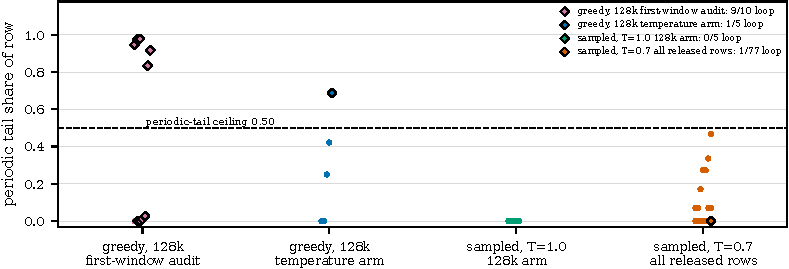
\includegraphics[width=0.95\linewidth]{figC_degeneracy.pdf}
\caption{Periodic tail share per row for the rows that ship with a per-row verdict, against
the 0.50 ceiling. Left and middle: greedy rows from two campaigns, 9 of 10 looping in the
first-window audit and 1 of 10 in the temperature arms. Right: every sampled row in the
release, old and fixed engines together, 1 of 83 looping. The long-context census that
motivated the move to sampling (9 of 15) is in Appendix~\ref{app:changes}; its per-row
sidecars are not part of this release, so it is quoted there and not used here.}
\label{fig:degeneracy}
\end{figure}

Three consequences are applied in this paper rather than merely noted. The headline protocol
is sampled at $T{=}0.7$, with the earlier greedy numbers reported separately and labelled. A
looping row is named wherever one appears, never smoothed into a mean. And the temperature
ablation points \emph{up}: at 128\,k, $T{=}1.0$ reaches acceptance 0.7369 against 0.4681 at
the headline $T{=}0.7$, with 0 of 5 rows degenerate in both arms.
% SRC: results/mlsys/RESULTS_OCT.md sections 1 and 8.5

\subsection{Rotary stretching: acceptance and perplexity dissociate}
\label{sec:res-rope}

The natural assumption is that an intervention which costs little in perplexity will cost
little in acceptance, because the draft and the target see the same positions. We tested it
on \texttt{meta-llama/Llama-3.1-8B} at 128\,k, with five books per arm and the arms differing
in nothing but \texttt{rope\_factor}.

\begin{table}[t]
\centering
\caption{The rotary intervention at 128\,k on \texttt{meta-llama/Llama-3.1-8B}: five books
per arm, seed 42, FP4 weights with an NF4 KV cache. The perplexity ratio is the paired
measurement against the native arm on the same continuation. The \texttt{tok/s} column is
\textbf{old-engine} throughput, reported for completeness only: the finding is the acceptance
and perplexity contrast, and no speedup is claimed from these arms.}
\label{tab:rope}
\begin{tabular}{lrrrr}
\toprule
Arm & $n$ & Acceptance & ppl ratio & tok/s \\
 & & & (vs native) & \emph{[old engine]} \\
\midrule
native & 5 & 0.7272 & 1.0000 & 0.9109 \\
factor 16 & 5 & 0.5336 & 1.0005 & 0.7699 \\
factor 32 & 5 & 0.5006 & 1.0156 & 0.7473 \\
\bottomrule
\end{tabular}

\end{table}

\begin{figure}[t]
\centering
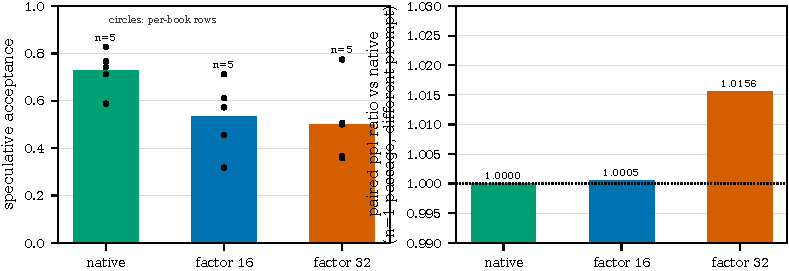
\includegraphics[width=0.95\linewidth]{figB_rope.pdf}
\caption{Left: speculative acceptance per arm, with the five books drawn as points so the
direction can be checked per book rather than only in the mean. Right: the paired perplexity
ratio against the native arm. Stretching the rotary basis costs $0.05\%$ and $1.56\%$ of
perplexity and $27\%$ and $31\%$ of acceptance.}
\label{fig:rope}
\end{figure}

Acceptance falls from \textbf{0.7272} (native) to \textbf{0.5336} (factor 16) and
\textbf{0.5006} (factor 32), a \textbf{27} to \textbf{31\%} relative loss, while the paired
perplexity ratio moves by \textbf{$+0.05\%$} and \textbf{$+1.56\%$}. The direction holds on
five books of five, so it is not a book effect, and because the arms differ in nothing else
the drop is a \textbf{rotary effect at $n{=}3$ arms}. The two stretched factors land far
closer to each other (6.6\% apart) than either lands to native, which is what a saturating
intervention looks like; at $n{=}3$ books their difference was 0.0012 and was read as exact
saturation, and at $n{=}5$ it is 0.033, so that specific reading is withdrawn and the weaker
claim stands.
% SRC: results/lcfy... see results/lcfm/CAMERA_READY_KIT.md F1; results/mlsys/sampling_session/session_a_ROPE_SAMP_*_SPEC.csv

A speculative decoder is only as good as the agreement between the draft's proposal
distribution and the target's. Position scaling is normally evaluated by perplexity, and by
that measure it is nearly free here. The same intervention costs almost a third of the
acceptance, and therefore almost a third of the speculation speedup, and nothing in the
perplexity number reveals it. Acceptance under any change to the target's positional
treatment has to be measured. One scope note: every arm here ran on the old engine, so the
absolute levels sit on the pre-fix decode path; the contrast is unaffected, because the fixed
kernel does not change which tokens are generated (\S\ref{sec:res-spec}).
% SRC: results/lcfm/CAMERA_READY_KIT.md F1

\subsection{Coherence at 1\,M on a natively long-context target}
\label{sec:res-coherence}

The perplexity comparison above cannot reach 1\,M, so we check the long-context property
directly on a target trained to 1\,M
(\texttt{gradientai/Llama-3-8B-Instruct-Gradient-1048k}), where nothing is being stretched and
the question is only whether the model is still a model. The rungs are matched by
\texttt{continuation\_sha256} and the recorded window offsets, never by a pool name.

On the \textbf{one exactly aligned book} the target's perplexity is \textbf{1.805 at 1\,M}
against \textbf{1.649 at 128\,k}, a \textbf{$+9.5\%$} move. On the two books that share 91 to
95\% of their scored tokens the difference is within \textbf{1.1\%}. So a natively
long-context target does stay coherent across an eightfold context increase, which is the
property the whole campaign depends on, but the strongest form of that claim rests on one
exactly aligned book and we say so rather than pooling three and reporting a tighter number.
The measurement is prefill-only, so the decode fix cannot move it: the numbers are identical
under both engines.
% SRC: results/mlsys/sampling_session/QUALITY_FIX_{128K,1M}_*; alignment.csv

\subsection{The ring's key/value rotation was the decode step}
\label{sec:res-decode}

At 128\,k, each decode token requires 8 rotations over 32 layers, so \textbf{256 rounds} of a
\texttt{batch\_isend\_irecv} ring per token. Figure~\ref{fig:ringbench} measures that
primitive with no model attached, over five payloads from 4\,KB to 266\,MB, the latter being
the key and value of a 128\,k window. Every payload costs the same ${\sim}10.3$\,ms: the range
spans 10.3124 to 10.3462\,ms, a 66{,}000$\times$ payload range with a \textbf{0.4\% spread}
and a worst rank-to-rank spread of 0.056\,ms over eight ranks. A round is latency, not
bandwidth, and it is paid once per round however small the round is. On the same box the
profiled ring path spent about 9.3\,ms per round, so the bare primitive accounts for the whole
cost of the decode step and leaves nothing to attribute to per-round engine overhead or rank
skew.
% SRC: results/mlsys/decode_df/ring_bench/ringbench.csv; results/mlsys/DECODE_DIAGNOSIS.md section F

\begin{figure}[t]
\centering
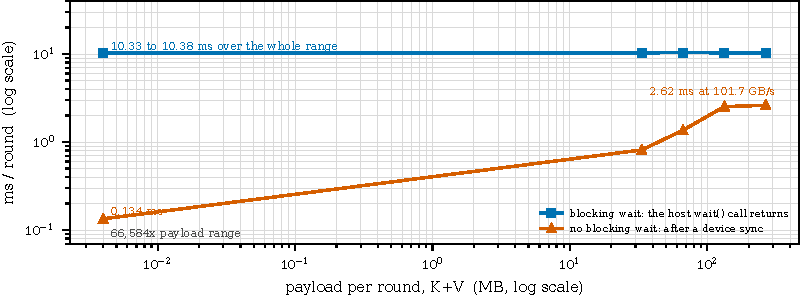
\includegraphics[width=0.62\linewidth]{figD_ring_bench.pdf}
\caption{A bare-process benchmark of the ring primitive the engine uses
(\texttt{batch\_isend\_irecv}, 8 ranks, 256 rounds per payload, no model). The line is flat: a
round costs a fixed ${\sim}10.3$\,ms from 4\,KB to 266\,MB, so the ring's decode cost is
per-round latency and cannot be amortised by moving more data per round. NCCL selected
\texttt{P2P/CUMEM/read} on a full NV12 mesh.}
\label{fig:ringbench}
\end{figure}

Removing the rotation is prior work (\S\ref{sec:related}), adopted here as \textbf{split-KV}:
each rank computes attention for the replicated query against only its own prefill shard,
producing a partial output and a log-sum-exp, and the partials are merged by one MAX and one
SUM all-reduce; for a single query token the partials are tiny and the replicated tail is
counted exactly once. Our contribution is the diagnosis and the measurement, not the
technique.

\begin{table}[t]
\centering
\caption{Decode time per token, old ring engine against split-KV, on \emph{matched}
(seed, book) cells: one value per cell on both sides, plumbing repeats dropped, and the two
seed stages hit by the configuration bug of \S\ref{sec:res-seeds} excluded. Speedup is the
ratio of decode-only times.}
\label{tab:headline}
\begin{tabular}{llrrrr}
\toprule
Context & Arm & \multicolumn{2}{c}{Decode s/token} & Speedup & $n$ \\
\cmidrule(lr){3-4}
 & & old ring & split-KV & & (cells) \\
\midrule
128k & spec & 1.4779 & \textbf{0.5275} & 2.80$\times$ & 3 \\
128k & target-only & 3.4925 & \textbf{1.0596} & 3.30$\times$ & 1 \\
512k & spec & 3.5344 & \textbf{0.9384} & 3.77$\times$ & 3 \\
512k & target-only & 9.9900 & \textbf{2.3460} & 4.26$\times$ & 1 \\
1M & spec & 6.0506 & \textbf{1.3830} & 4.38$\times$ & 13 \\
1M & target-only & 17.0902 & \textbf{3.2107} & 5.32$\times$ & 2 \\
\bottomrule
\end{tabular}

\end{table}

\begin{figure}[t]
\centering
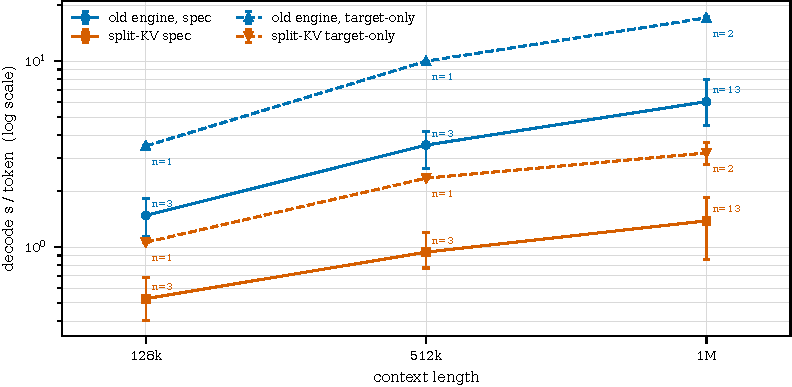
\includegraphics[width=0.92\linewidth]{figA_decode_vs_context.pdf}
\caption{Decode time per token against context length, both engines and both arms, on the
same matched cells. Whiskers are the range over cells and $n$ is the number of cells both
engines measured. The gap widens with context, which is the signature of a
context-independent per-round cost being removed from a step whose other terms grow.}
\label{fig:decode-context}
\end{figure}

Table~\ref{tab:headline} and Figure~\ref{fig:decode-context} are the headline. Decode-only,
the fix is worth \textbf{2.80$\times$ / 3.77$\times$ / 4.37$\times$} with speculation and
\textbf{3.30$\times$ / 4.26$\times$ / 5.32$\times$} without it at 128\,k / 512\,k / 1\,M, and
\textbf{the speedup grows with context}, which is the mechanistic claim rather than a
by-product: as the rest of the decode step grows with the context, the rotation's fixed share
of it shrinks relative to the rotation-free path that replaces it, so the ratio improves. Two
caveats we state rather than bury. The matched old-against-new comparison is one cell at
512\,k and two at 1\,M, because that is how many books the old engine measured there, while
the fixed engine's own target-only arms were widened from one and two books to three and five
by a later top-up run. And the four diagnostic arms that isolated the mechanism,
\texttt{kv\_block\_size} 32768 ($1.24\times$) and \texttt{repeat\_kv} after the rotation
($+2.7\%$), are bit-identical in token stream and inert under split-KV, so they carry no claim
here; they are reported because they ruled out the cheaper explanations first.
% SRC: results/mlsys/RESULTS_OCT.md sections 10.2a, 10.2b, 10.7; results/mlsys/decode_df/arms/df_arms.csv

\subsection{Speculation still pays, and the baseline is corrected}
\label{sec:res-spec}
\label{sec:res-seeds}

With the rotation gone, the question the paper started from can be asked on an engine whose
decode step is no longer dominated by a collective. The answer is yes:
\textbf{2.01$\times$ / 2.29$\times$ / 2.20$\times$} decode-only at 128\,k / 512\,k / 1\,M over
the same engine's own target-only path, with three books against one in the 128\,k arms, three
against three at 512\,k, and five against five at 1\,M. End-to-end, where prefill is included,
the same comparison reads $1.95\times$ / $1.76\times$ / $1.41\times$, because at 1\,M a row is
570\,s of which about 340\,s is prefill: with the decode step fixed, prefill is the long pole
and any statement about 1\,M throughput has to say which of the two it means.
% SRC: results/mlsys/RESULTS_OCT.md sections 10.2 and 10.7

Two of those denominators used to be one and two books. We topped them up after the
confirmatory run, because a ratio whose denominator is one row is a ratio of one row to
another. The 512\,k target-only mean is $2.148$\,s/token over three books against the $2.346$
single-book value it replaces, and the 1\,M mean is $3.155$ over five against $3.211$ over
two. Both moves are downward, so the quoted ratios are lower than the thin ones: the thin
denominator was flattering, by $8\%$ at 512\,k. The book-to-book spread inside the fixed
engine is 1.27$\times$ at 512\,k and 1.30$\times$ at 1\,M, wider than the 1.04$\times$ spread
across seeds, so books and seeds are not interchangeable units.
% SRC: results/mlsys/rerun_topup/session_a_TP_*.csv; results/mlsys/RESULTS_OCT.md sections 10.3, 10.7

\paragraph{The corrected old-engine baseline.} Two stages of the seed ablation, the ones meant
to run seeds 123 and 456 at 1\,M, ran seed 42 instead, because the config builder merges a
level into the defaults and then sets the seed from the \emph{defaults'} list, so a level that
declares its own \texttt{seeds} has it recorded and overwritten. Rebuilt from rows that were
never affected, on 13 matched (seed, book) cells, the 1\,M speedup is \textbf{4.375$\times$}
rather than $4.033\times$ and the 1\,M acceptance difference is \textbf{$-0.1\%$} rather than
$-10.4\%$: the fixed engine's acceptance is \emph{unchanged}, and the previously reported drop
was the bug. The old engine's own seed spread is 23.0\% of the mean on the matched books, so
per-seed movement of $-15.7\%$, $+10.9\%$ and $+11.3\%$ sits inside the old engine's own
seed-to-seed variation, in both directions.
% SRC: scripts/mlsys_seed_baseline_audit.py; results/mlsys/RESULTS_OCT.md section 10.3

\paragraph{The speedups are not bought with a different model.} An exactly equivalent kernel
can still move an acceptance number, because the accept/reject decision compares the target's
distribution against the draft's proposal, so one flipped near-tie changes the emitted prefix
and every later proposal with it. We checked the kernel directly: the target-only stream under
split-KV is \textbf{bit-identical to the ring baseline for twelve consecutive tokens} and
diverges at a step where the baseline's own top-2 logit margin is \textbf{0.0000}, against a
row median of 2.9375, with prefill perplexity identical to six decimals.
% SRC: results/mlsys/DECODE_DIAGNOSIS.md sections F.4/F.5

\subsection{Comparison against a production engine}
\label{sec:res-vllm}

We benchmark vLLM 0.6.3 at tensor-parallel 8 on the same prompts, fed the same token ids from
our own sidecars, so the units match. The comparison is \textbf{not precision-matched}: vLLM
runs \textbf{bf16 weights with a bf16 KV cache and greedy decoding}, while RASD runs
\textbf{FP4 weights with an NF4 KV cache} at $T{=}0.7$ with speculation. Every ratio below
carries that mismatch.

\begin{table}[t]
\centering
\caption{vLLM (bf16, bf16 KV, greedy) against the ring engine and the split-KV engine (FP4
weights, NF4 KV, $T{=}0.7$ sampled) on the same prompts. Prefill is the first-token time and
decode is per token. \textbf{Not a precision-matched comparison}: the systems differ in
precision and in sampling.}
\label{tab:vllm}
\begin{tabular}{lrrrrrr}
\toprule
 & \multicolumn{2}{c}{Prefill (s)} & \multicolumn{2}{c}{vLLM run /} & \multicolumn{2}{c}{Decode (s/token)} \\
\cmidrule(lr){2-3}\cmidrule(lr){4-5}\cmidrule(lr){6-7}
Context & vLLM & RASD & RASD prefill & RASD prefill & vLLM & RASD split-KV \\
 & & & \multicolumn{2}{c}{(same quantity)} & & \\
\midrule
128k & 16.85 & 8.76 & 1.92$\times$ & 2.04$\times$ & 0.0081 & 1.06 \\
512k & 222.80 & 88.56 & 2.52$\times$ & 2.54$\times$ & 0.0145 & 2.35 \\
1M & 859.60 & 335.34 & 2.56$\times$ & 2.57$\times$ & 0.0234 & 3.21 \\
\bottomrule
\end{tabular}

\end{table}

Two readings that point in opposite directions, and both belong here. \textbf{Our prefill
beats vLLM's entire run}, meaning its prefill plus its 128 decode steps, by $1.92\times$ /
$2.52\times$ / $2.56\times$ at 128\,k / 512\,k / 1\,M; that is a property of the ring prefill,
untouched by the decode fix, and it is the strongest end-to-end statement this paper can make
against a production engine. And \textbf{vLLM's decode is 130 to 162$\times$ faster per token
than ours even after the fix}, against 429 to 731$\times$ before it: removing the rotation
eliminated roughly $70\%$ of the decode deficit and left our decode far behind a production
engine. Speculation does not close the gap either, since our spec decode is $65\times$,
$65\times$ and $59\times$ vLLM's. The honest framing is that the ring's rotation was the
decode \emph{pathology}, and removing it made our decode merely slow.
% SRC: results/mlsys/vllm_run2/vllm_baseline.csv; results/lcfm/CAMERA_READY_KIT.md section 3d

\section{Limitations}
\label{sec:limitations}

\begin{itemize}[leftmargin=*,topsep=2pt,itemsep=1pt]
  \item \textbf{Sample size.} The matched comparison is 3 spec and 1 target-only cell at
        128\,k, 3 and 1 at 512\,k, 13 and 2 at 1\,M. Inside the fixed engine the target-only
        arms are 1, 3 and 5 books. The five units in a five-book arm are books, not seeds, and
        the book spread is wider than the seed spread.
  \item \textbf{The draft saw the prompt's first 4096 tokens} (\S\ref{sec:setup}), so every
        acceptance level here is a lower bound; contrasts between arms are unaffected.
  \item \textbf{One node, one fabric, one precision.} Everything is 8$\times$A100 80\,GB SXM4
        over NVLink. Multi-node moves the collective to a slower fabric, which is exactly the
        regime where per-round latency, the quantity \S\ref{sec:res-decode} measures, grows.
        There is no bf16 row: every number carries the FP4/NF4 precision cost.
  \item \textbf{Acceptance under split-KV is explained, not tested.} The 1\,M acceptance is
        unchanged over 13 matched cells while per seed it moves both ways inside a 23.0\%
        old-engine spread. The mechanism we offer, one flipped near-tie changing the emitted
        prefix, is consistent with every measurement and was not tested directly.
  \item \textbf{Prefill is now the 1\,M pole}: a 1\,M row is 570\,s of which about 340\,s is
        prefill, so the end-to-end 1\,M speedup is $1.41\times$ against $2.20\times$
        decode-only.
  \item \textbf{An unattributed elementwise term.} In the profiled 128\,k decode window,
        19.3\% of device time was elementwise kernels never attributed to an operation. With
        the rotation gone that is a larger share of what remains, and it is the obvious next
        optimisation.
  \item \textbf{Two withdrawn claims are recorded rather than deleted} (Appendix
        \ref{app:changes}): the reviewed version's ``communication is at most $1.2\%$ of wall
        time'', whose bucket recorded 0.31 to 0.37$\times$ of the physical floor for the same
        runs, and the $4.4\times$ ``native context'' speedup from one pair in one session.
\end{itemize}

\section{Conclusion}
\label{sec:conclusion}

We asked what limits speculative decoding at a million tokens, and the answer arrived in three
parts, none of them about speculation itself. Under greedy decoding the acceptance numbers
this kind of campaign reports are measured on degenerate text: 9 of 10 long-context rows in
the released first-window audit loop, and 1 of 83 sampled rows does. Once the protocol is
sampled at $T{=}0.7$, stretching a model's rotary basis costs a quarter of the acceptance
($27$ to $31\%$ relative) for $0.05$ to $1.56\%$ of perplexity, so acceptance and perplexity
dissociate and the second cannot stand in for the first. A natively 1M-trained target stays
coherent at 1\,M, within $9.5\%$ of its own 128\,k perplexity on the exactly aligned book, so
the regime is not intrinsically hostile to speculation.

What was hostile was our engine. Rotating each layer's key/value shard around eight ranks
costs 256 rounds per decode token, and a bare-process benchmark shows each round costs a fixed
${\sim}10.3$\,ms whatever the payload, from 4\,KB to 266\,MB within $0.4\%$: the decode step
was latency per round. Adopting decode-side context parallelism, which is prior work, removes
those rounds and is worth $2.80$ to $4.37\times$ decode-only with speculation and $3.30$ to
$5.32\times$ without it, growing with context as a context-independent per-round cost
predicts, while speculation still pays $2.01$ to $2.29\times$ on top and the matched 1\,M
acceptance is unchanged at $-0.1\%$. Against vLLM at bf16 with greedy decoding, which is not a
precision-matched comparison, our prefill beats its entire run by $1.92$ to $2.56\times$ and
its decode remains $130$ to $162\times$ faster per token than ours. The rotation was the
decode pathology; removing it made our decode merely slow. That is the honest systems claim,
and it is the one this paper makes.

% References come before the appendices, as the style expects, so that the
% page check measures the main text and not the appendix.
\bibliographystyle{plainnat}
\bibliography{references}

\appendix

\section{Changes from the reviewed version}
\label{app:changes}

Every claim in the reviewed submission, with its status here. Corrections cite the audit item
that found them (\path{results/mlsys/LCFM_RECONCILE.md}, AUDIT E1 to E23).

\begin{table}[h]
\centering\footnotesize
\caption{Status of every claim in the reviewed version. KEPT means it stands as written;
CORRECTED gives the old reading and the new one; REMOVED means the claim is withdrawn and not
replaced. Audit items are E1 to E23 of \texttt{results/mlsys/LCFM\_RECONCILE.md}.}
\label{tab:changes}
\setlength{\tabcolsep}{4pt}
\begin{tabular}{p{0.30\linewidth} p{0.115\linewidth} p{0.505\linewidth}}
\toprule
Claim in the reviewed version & Status & Reason \\
\midrule
Communication at most $1.2\%$ of wall (E1) & REMOVED & The bucket recorded 0.31 to 0.37$\times$ of the physical wire floor, so it never saw the transfers. \\
Idle at or above $50\%$ is collective wait (E2) & REMOVED & Measured outside the region the collectives run in. \\
The tick-gate barrier (E3) & REMOVED & Not the code that produced the reported numbers. \\
The rotation is hidden and the draft pass is free (E4) & CORRECTED & The rotation is issued before attention, and the claimed draft overlap was never implemented. \\
Positioning table and novelty framing (E5) & CORRECTED & Split-KV is prior work, and the decode-overlap cell was not implemented. \\
The draft saw the last 4096 tokens (E6) & CORRECTED & It saw the first 4096, on every run whose prompt exceeded that (\texttt{d89cf41}). \\
Anchor is the model's original window (E7) & CORRECTED & Each context was anchored on its own length. \\
Factor $\lceil N/4096\rceil$ (E8, E9) & CORRECTED & A fixed factor 8 at 8\,k and above, and none below. \\
Verify-loop defects (E10) & CORRECTED & Per AUDIT E10. \\
Three independent seed samples (E11) & CORRECTED & All three seeds ran one prompt. \\
$95\%$ intervals at $n{=}3$ (E12) & CORRECTED & Ranges are reported, with the $n$. \\
Nominal 1\,M context (E13) & CORRECTED & 1{,}047{,}551 prompt tokens here against 1{,}002{,}984 in the reviewed build. \\
Speedup regresses to $0.94\times$ and $0.97\times$ (E14) & REMOVED & Decode tokens per round are flat, and the same-code rerun does not reproduce it. \\
A control explains the bimodality (E15) & REMOVED & The control differs from the long-context cells in five ways at once. \\
$4.4\times$ at native context (E16) & REMOVED & One pair in one session, above what its own acceptance can deliver. \\
The speedup formula (E17) & CORRECTED & Applied to the wrong quantity; throughput is tokens over time. \\
Peak memory per rank (E18) & CORRECTED & The peak was rank 0 only; over ranks it is 41.2\,GiB allocated. \\
``NF4 weights'' (E19) & CORRECTED & The weights are FP4; NF4 is the KV codec. \\
NF4 KV description (E20) & CORRECTED & Per AUDIT E20. \\
Design-point sweeps (E21) & CORRECTED & Chunk size does not bound memory, depth 2 repeats depth 1, and the $\gamma$ optimum is unsupported. \\
Prompts and citations (E22) & CORRECTED & The synthetic prompt is not the prior-work protocol, and one citation does not exist. \\
Qualitative comparison (E23) & KEPT & Stands, with the audit's caveat. \\
Greedy census, 9 of 15 rows looping & KEPT, MOVED HERE & Its per-row sidecars are \textbf{not released}, so the main text quotes released numbers only. \\
Profiler time-breakdown table and figure & CUT & The comm bucket in it is below the physical floor, so it bounds nothing. \\
Llama-2 quantization and rotary perplexity table & CUT & Labelled by intent rather than configuration, and one claim cited a number that does not exist. \\
RULER infrastructure appendix & CUT & Infrastructure without a run grid supports no claim. \\
\bottomrule
\end{tabular}
\end{table}

\section{The corrected baseline and the matched-cell tables}
\label{app:baseline}

\begin{table}[h]
\centering\footnotesize
\caption{Decode time per token on matched (seed, book) cells, one value per cell on both
sides, plumbing repeats dropped, bug-affected seed stages excluded. This is the table the main
text quotes.}
\label{tab:matched}
\begin{tabular}{llrrrr}
\toprule
Context & Arm & \multicolumn{2}{c}{Decode s/token} & Speedup & $n$ \\
\cmidrule(lr){3-4}
 & & old ring & split-KV & & (cells) \\
\midrule
128k & spec & 1.4779 & \textbf{0.5275} & 2.80$\times$ & 3 \\
128k & target-only & 3.4925 & \textbf{1.0596} & 3.30$\times$ & 1 \\
512k & spec & 3.5344 & \textbf{0.9384} & 3.77$\times$ & 3 \\
512k & target-only & 9.9900 & \textbf{2.3460} & 4.26$\times$ & 1 \\
1M & spec & 6.0506 & \textbf{1.3830} & 4.38$\times$ & 13 \\
1M & target-only & 17.0902 & \textbf{3.2107} & 5.32$\times$ & 2 \\
\bottomrule
\end{tabular}

\end{table}

\paragraph{The configuration bug.} \path{run_experiment.py:590-612} merges a level into the
defaults and then sets the run's seed from the \emph{defaults'} \texttt{seeds} list, so a level
that declares its own \texttt{seeds} has it recorded and then overwritten. Exactly two stages
did: \texttt{SA\_SEED\_123\_1M\_SPEC} and \texttt{SA\_SEED\_456\_1M\_SPEC}, both of which ran
seed 42 while their run ids said otherwise. Every old-engine pool containing them inherited
the error. The corrected baseline is built from rows that were never affected, seed 42 from
the sampling session and seeds 123 and 456 from a dedicated rerun; the exclusion list is
printed by \path{scripts/mlsys_seed_baseline_audit.py} and reproduced in
\path{results/mlsys/SEED_BASELINE_AUDIT.txt}.

\begin{table}[h]
\centering\footnotesize
\caption{The corrected old-engine baseline at 1\,M, over the 13 matched (seed, book) cells
where both engines have a row. The old engine's spread across its own seeds is 23.0\% of the
mean on these books.}
\label{tab:seedbias}
\begin{tabular}{lrrr}
\toprule
seed & old acceptance & fixed-engine acceptance & change \\
\midrule
42  & 0.5246 & 0.4424 & $-15.7\%$ \\
123 & 0.4656 & 0.5164 & $+10.9\%$ \\
456 & 0.4466 & 0.4969 & $+11.3\%$ \\
\midrule
pooled over 13 cells & 0.4839 & 0.4834 & $-0.1\%$ \\
\bottomrule
\end{tabular}
\end{table}

\begin{table}[h]
\centering\footnotesize
\caption{The target-only top-up. The fixed engine's own target-only arms were widened after
the confirmatory run; the matched old-against-new cells are unchanged by it.}
\label{tab:topup}
\begin{tabular}{llrrl}
\toprule
stage & book & context & decode s/token & provenance \\
\midrule
\texttt{TP\_GATE\_128K\_TARGET} & \texttt{train\_0} & 128\,k & 1.051 & \texttt{split\_kv}, 32 layers \\
\texttt{TP\_1M\_TARGET} & \texttt{train\_915} & 1\,M & 2.826 & \texttt{split\_kv}, 32 layers \\
\texttt{TP\_1M\_TARGET} & \texttt{train\_2204} & 1\,M & 3.126 & \texttt{split\_kv}, 32 layers \\
\texttt{TP\_1M\_TARGET} & \texttt{train\_2768} & 1\,M & 3.402 & \texttt{split\_kv}, 32 layers \\
\texttt{TP\_512K\_TARGET} & \texttt{train\_1} & 512\,k & 1.847 & \texttt{split\_kv}, 32 layers \\
\texttt{TP\_512K\_TARGET} & \texttt{train\_915} & 512\,k & 2.251 & \texttt{split\_kv}, 32 layers \\
\bottomrule
\end{tabular}
\end{table}

\paragraph{Effect.} The 512\,k target-only mean moves from 2.3460 over one book to 2.1480 over
three, and the 1\,M mean from 3.2107 over two books to 3.1553 over five. The spec-over-target
ratios in \S\ref{sec:res-spec} are computed on these wider arms; the matched speedups in
Table~\ref{tab:matched} are not affected, because the new books have no old-engine
counterpart. Both movements are downward, so widening the denominator lowered the reported
ratios rather than raising them.
% SRC: results/mlsys/rerun_topup/session_a_TP_*.csv

\section{The decode diagnosis in detail}
\label{app:diagnosis}

\begin{table}[h]
\centering\footnotesize
\caption{Bare-process ring benchmark: the \texttt{batch\_isend\_irecv} ring primitive the
engine uses, 8 ranks, 256 rounds per payload, no model attached. Reported for rank 0; the
worst rank-to-rank spread over all eight ranks is 0.056\,ms.}
\label{tab:bench}
\begin{tabular}{lrrrr}
\toprule
payload & size & K+V bytes & ms/round & GB/s \\
\midrule
\texttt{tiny\_4kb}   & 4\,KB      & 4{,}096      & \textbf{10.3124} & 0.0 \\
\texttt{mb33}        & 33.3\,MB   & 34{,}918{,}400 & 10.3437 & 3.22 \\
\texttt{k8\_66mb}    & 66.6\,MB   & 69{,}836{,}800 & 10.3389 & 6.44 \\
\texttt{mb133}       & 133.2\,MB  & 139{,}673{,}600 & 10.3557 & 12.86 \\
\texttt{mb266}       & 266.3\,MB  & 279{,}347{,}200 & \textbf{10.3462} & 25.74 \\
\bottomrule
\end{tabular}
\end{table}

The five payloads span a factor of 66{,}000 in bytes and 0.4\% in time, so the round is
dominated by fixed latency and not by transfer. This is why the fix is to remove the rounds
rather than to move more data per round.

\begin{table}[h]
\centering\footnotesize
\caption{The engine arms: one model load, four configurations, 128\,k target-only at 16
tokens each. The two ring variants are bit-identical in token stream to \texttt{ring2048} and
the split-KV kernel is bit-identical to \texttt{ring32768} for twelve tokens.}
\label{tab:arms}
\begin{tabular}{lrrrr}
\toprule
configuration & target-only s/token & vs \texttt{ring2048} & vs \texttt{ring32768} & token stream \\
\midrule
\texttt{ring2048}   & 3.5637 & 1.000$\times$ & & baseline \\
\texttt{ring32768}  & 2.8749 & 1.240$\times$ & 1.000$\times$ & bit-identical \\
\texttt{ring32768x} & 2.7985 & 1.273$\times$ & 1.027$\times$ & bit-identical \\
\texttt{splitkv}    & \textbf{1.0011} & \textbf{3.560$\times$} & \textbf{2.872$\times$} & 12 tokens, then a tie \\
\bottomrule
\end{tabular}
\end{table}

\paragraph{Correctness.} The target-only stream under split-KV is bit-identical to the ring
baseline for twelve consecutive tokens and then diverges at a step where the baseline's own
top-2 logit margin is \textbf{0.0000}, against a row median of 2.9375 and a minimum of 0.0000:
an exact tie broken the other way. Greedy repeats the pattern, and the speculative row
diverges at index 1 with margin 0.8750 against a row median of 0.9375, below the row's own
median. Prefill perplexity is identical to six decimals under both configurations, and the
perplexity gate is in any case blind to a decode-path change, because it scores a prefill
forward with \texttt{use\_cache=False}.
% SRC: results/mlsys/DECODE_DIAGNOSIS.md sections F.4/F.5; results/mlsys/decode_df/arms/df_arms.csv

\section{Ablations kept from the reviewed version}
\label{app:ablations}

The design-point sweeps are \textbf{old-engine} results on the \textbf{synthetic repeated
paragraph} at 64\,k on 8$\times$A100 40\,GB, three seeds on one prompt, so the bracketed
figures are ranges over those three runs and not confidence intervals. They are kept because
they document how the system's knobs were chosen, and because two of the reviewed version's
readings of them were wrong: the chunk size is a transmission chunk and does not bound memory,
and prefetch depth 2 executes the same code path as depth 1, so that axis had two arms and not
three. The block-size effect is specific to the ring decode path and is inert under split-KV.

{\footnotesize\setlength{\tabcolsep}{4pt}\begin{table}[h]
\centering
\caption{M3 ablation results (64\,k context, 8$\times$A100-SXM4-40\,GB). Mean and range over 3 seeds: \textbf{three seeds on one synthetic prompt}, not three independent samples, so the bracketed intervals are ranges rather than confidence intervals (AUDIT E11, E12); horizontal rules separate the five sweep axes. Deterministic early-EOS rows with tokens\_generated $<$ 20 are excluded; see \S\ref{app:ablations} in this paper for the exclusion rule.}
\label{tab:m3-ablation}
\small\setlength{\tabcolsep}{3pt}\begin{tabular}{p{3.05cm}p{2.15cm}rrr}
\toprule
Axis & Level & Throughput (tok/s) [range] & Accept.\ [range] & $n$ \\
\midrule
A1: Draft model & TinyLlama-1.1B & 0.84 [0.82, 0.85] & 0.235 [0.226, 0.252] & 3 \\
 & Sheared-1.3B & 0.87 [0.84, 0.90] & 0.253 [0.231, 0.277] & 3 \\
\midrule
A2: Spec steps (k) & k=2 & 0.81 [0.74, 0.85] & 0.381 [0.303, 0.424] & 3 \\
 & k=4 & 0.86 [0.81, 0.91] & 0.253 [0.231, 0.277] & 3 \\
 & k=6 & 0.84 [0.80, 0.88] & 0.176 [0.149, 0.193] & 3 \\
 & k=8 & 0.86 [0.80, 0.89] & 0.147 [0.124, 0.160] & 3 \\
 & k=12 & 0.85 [0.82, 0.88] & 0.111 [0.105, 0.119] & 3 \\
\midrule
A3: KV block size & 256 & 0.62 [0.58, 0.65] & 0.253 [0.231, 0.277] & 3 \\
 & 512 & 0.87 [0.81, 0.93] & 0.253 [0.231, 0.277] & 3 \\
 & 1024 & 1.11 [1.06, 1.15] & 0.253 [0.231, 0.277] & 3 \\
 & 2048 & 1.25 [1.20, 1.30] & 0.253 [0.231, 0.277] & 3 \\
\midrule
A4: Prefetch depth & sync & 0.88 [0.84, 0.90] & 0.253 [0.231, 0.277] & 3 \\
 & async-1 & 0.87 [0.81, 0.92] & 0.253 [0.231, 0.277] & 3 \\
 & async-2 & 0.86 [0.84, 0.89] & 0.253 [0.231, 0.277] & 3 \\
\midrule
A5: Target model & Llama-2-7B & 0.86 [0.83, 0.90] & 0.253 [0.231, 0.277] & 3 \\
\bottomrule
\end{tabular}
\end{table}
}

\section{Reproduction and evidence tree}
\label{app:evidence}

\paragraph{Where every number lives.} Nothing in this paper is transcribed by hand. The
figures and tables are written by \path{scripts/lcfm_figures.py}, which reads the CSVs below
and writes \path{results/lcfm/figs/} and \path{results/lcfm/tables/}; those tables are
\emph{included} by this document rather than copied into it.

\begin{itemize}[leftmargin=*,topsep=2pt,itemsep=1pt]
  \item \textbf{Rotary intervention} \path{results/mlsys/sampling_session/session_a_ROPE_SAMP_*_SPEC.csv}
        and \path{results/mlsys/n5_extension/session_a_ROPE_EXT_*}, with the paired
        perplexity ratios in \path{session_a_rope_fix_gate.csv}.
  \item \textbf{Degeneracy} the per-stage \path{repetition_*.csv}, produced by
        \path{scripts/mlsys_repetition_report.py} from the token sidecars with the ceilings
        in \path{src/analysis/repetition.py}; where no such CSV exists the row is scored from
        the sidecar by the same module.
  \item \textbf{Coherence} \path{QUALITY_FIX_{128K,1M}_*} with the alignment table
        \path{results/mlsys/sampling_session/alignment.csv}.
  \item \textbf{The decode fix} the confirmatory run in \path{results/mlsys/rerun_r1/} and
        \path{rerun_r2/} (31 ok rows, each recording its engine and commit), the diagnostic
        arms in \path{results/mlsys/decode_df/arms/df_arms.csv}, and the top-up in
        \path{results/mlsys/rerun_topup/}.
  \item \textbf{The bare ring} \path{results/mlsys/decode_df/ring_bench/ringbench.csv}, from
        \path{scripts/mlsys_ring_microbench.py}.
  \item \textbf{The corrected baseline} \path{scripts/mlsys_seed_baseline_audit.py}, which
        prints the exclusion list and the matched-cell table.
  \item \textbf{vLLM reference} \path{results/mlsys/vllm_run2/vllm_baseline.csv} (bf16, bf16
        KV, greedy, unit-matched on every row). The earlier run at
        \path{results/mlsys/vllm_run/} is retained but its first-token and decode clocks are
        absolute monotonic readings and are unusable; only its end-to-end numbers agree,
        within 2.4\% at 128\,k and 0.1\% elsewhere.
\end{itemize}

\paragraph{The ceiling test, in one place.} Vanilla HuggingFace \texttt{generate()} with
FlashAttention-2, bf16 weights and a bf16 KV cache, single rank, no quantization and no
sequence parallelism, on \texttt{meta-llama/Llama-2-7b-hf}: 32\,k completes at 30.1\,GiB and
7.25\,tok/s, and every context of 128\,k and above runs out of memory during prefill. The
model differs from the targets used for the throughput results (\S\ref{sec:setup}), so this is
a capability reference for the standard stack and nothing more; no ratio in this paper uses
it.
% SRC: results/mlsys/RESULTS_OCT.md section 5.1; results/baselines/hf_ceiling.csv

\paragraph{Building this paper.} \texttt{cd manuscript/lcfm} and compile \texttt{main.tex} with
\texttt{latexmk} or \texttt{tectonic}; the bibliography is \texttt{references.bib}. The long
version of this work, including the withdrawn material and the full Ablations, lives in
\path{manuscript/arxiv/}.

\end{document}
